%! TEX program = lualatex
\documentclass[12pt,a4paper]{article} 

% Packages for formatting
\usepackage{fontspec}
\usepackage[ngerman]{babel}
\usepackage{geometry} 
\geometry{margin=1in} 
\usepackage{setspace} 
\usepackage{hyperref} 
\usepackage{xcolor}
\usepackage{amsmath} % for align*
\usepackage{amsthm} % neue Theorem-Umgebungen
\usepackage{enumitem} % für schöne Listen (Teilaufgaben)
\usepackage{mathbbol}
\usepackage{graphicx}
\usepackage{amssymb}
\usepackage{gensymb}

% Style settings
%\pagecolor{black}      % sets background color to black 
%\color{white}          % sets text color to white

% Change subsection to use a, b, c instead of 1, 2, 3
\renewcommand{\thesubsection}{\alph{subsection})} 

% Aufgaben-Umgebung definieren 
\newtheorem{aufgabe}{Aufgabe}

% Title page info 
\title{Blatt 03} 
\author{Hannes Rall \\ Albert-Ludwigs-University} 
\date{\today} 

\begin{document} 
% Title page 
\begin{titlepage}     
    \centering     
    \vspace*{2cm}     
    {\Huge\itshape Blatt 03\par}     
    \vspace{2cm}     
    {\Large\textsc{Hannes Rall}\par}     
    \vfill     
    {\large Albert-Ludwigs-University\\}     
    \vspace{1cm}     
    {\large\today\par}
\end{titlepage}

\newpage
\section*{Aufgabe 7}
\subsection*{(i)}
Sei $\triangle ABC$ ein gleichseitiges Dreieck mit Seitenlänge $a$. Die Seite $AC$ sei als Grundseite gewählt. Die Höhe $h$ des Dreiecks steht senkrecht auf $AC$ und verläuft durch den gegenüberliegenden Eckpunkt $B$. Betrachte nun einen Punkt $D$ auf der Seite $AB$. Von $D$ aus werden zwei Strecken:

Die Strecke $x$ ist die Senkrechte von $AC$ durch $D$.

Die Strecke $y$ ist die Senkrechte von $BC$ durch $D$.\\
Dann gilt: h=x+y (Wobei hier die Länge der Strecken gemeint ist).
\subsection*{(ii)}
\begin{figure}[htbp]        
    \centering        
    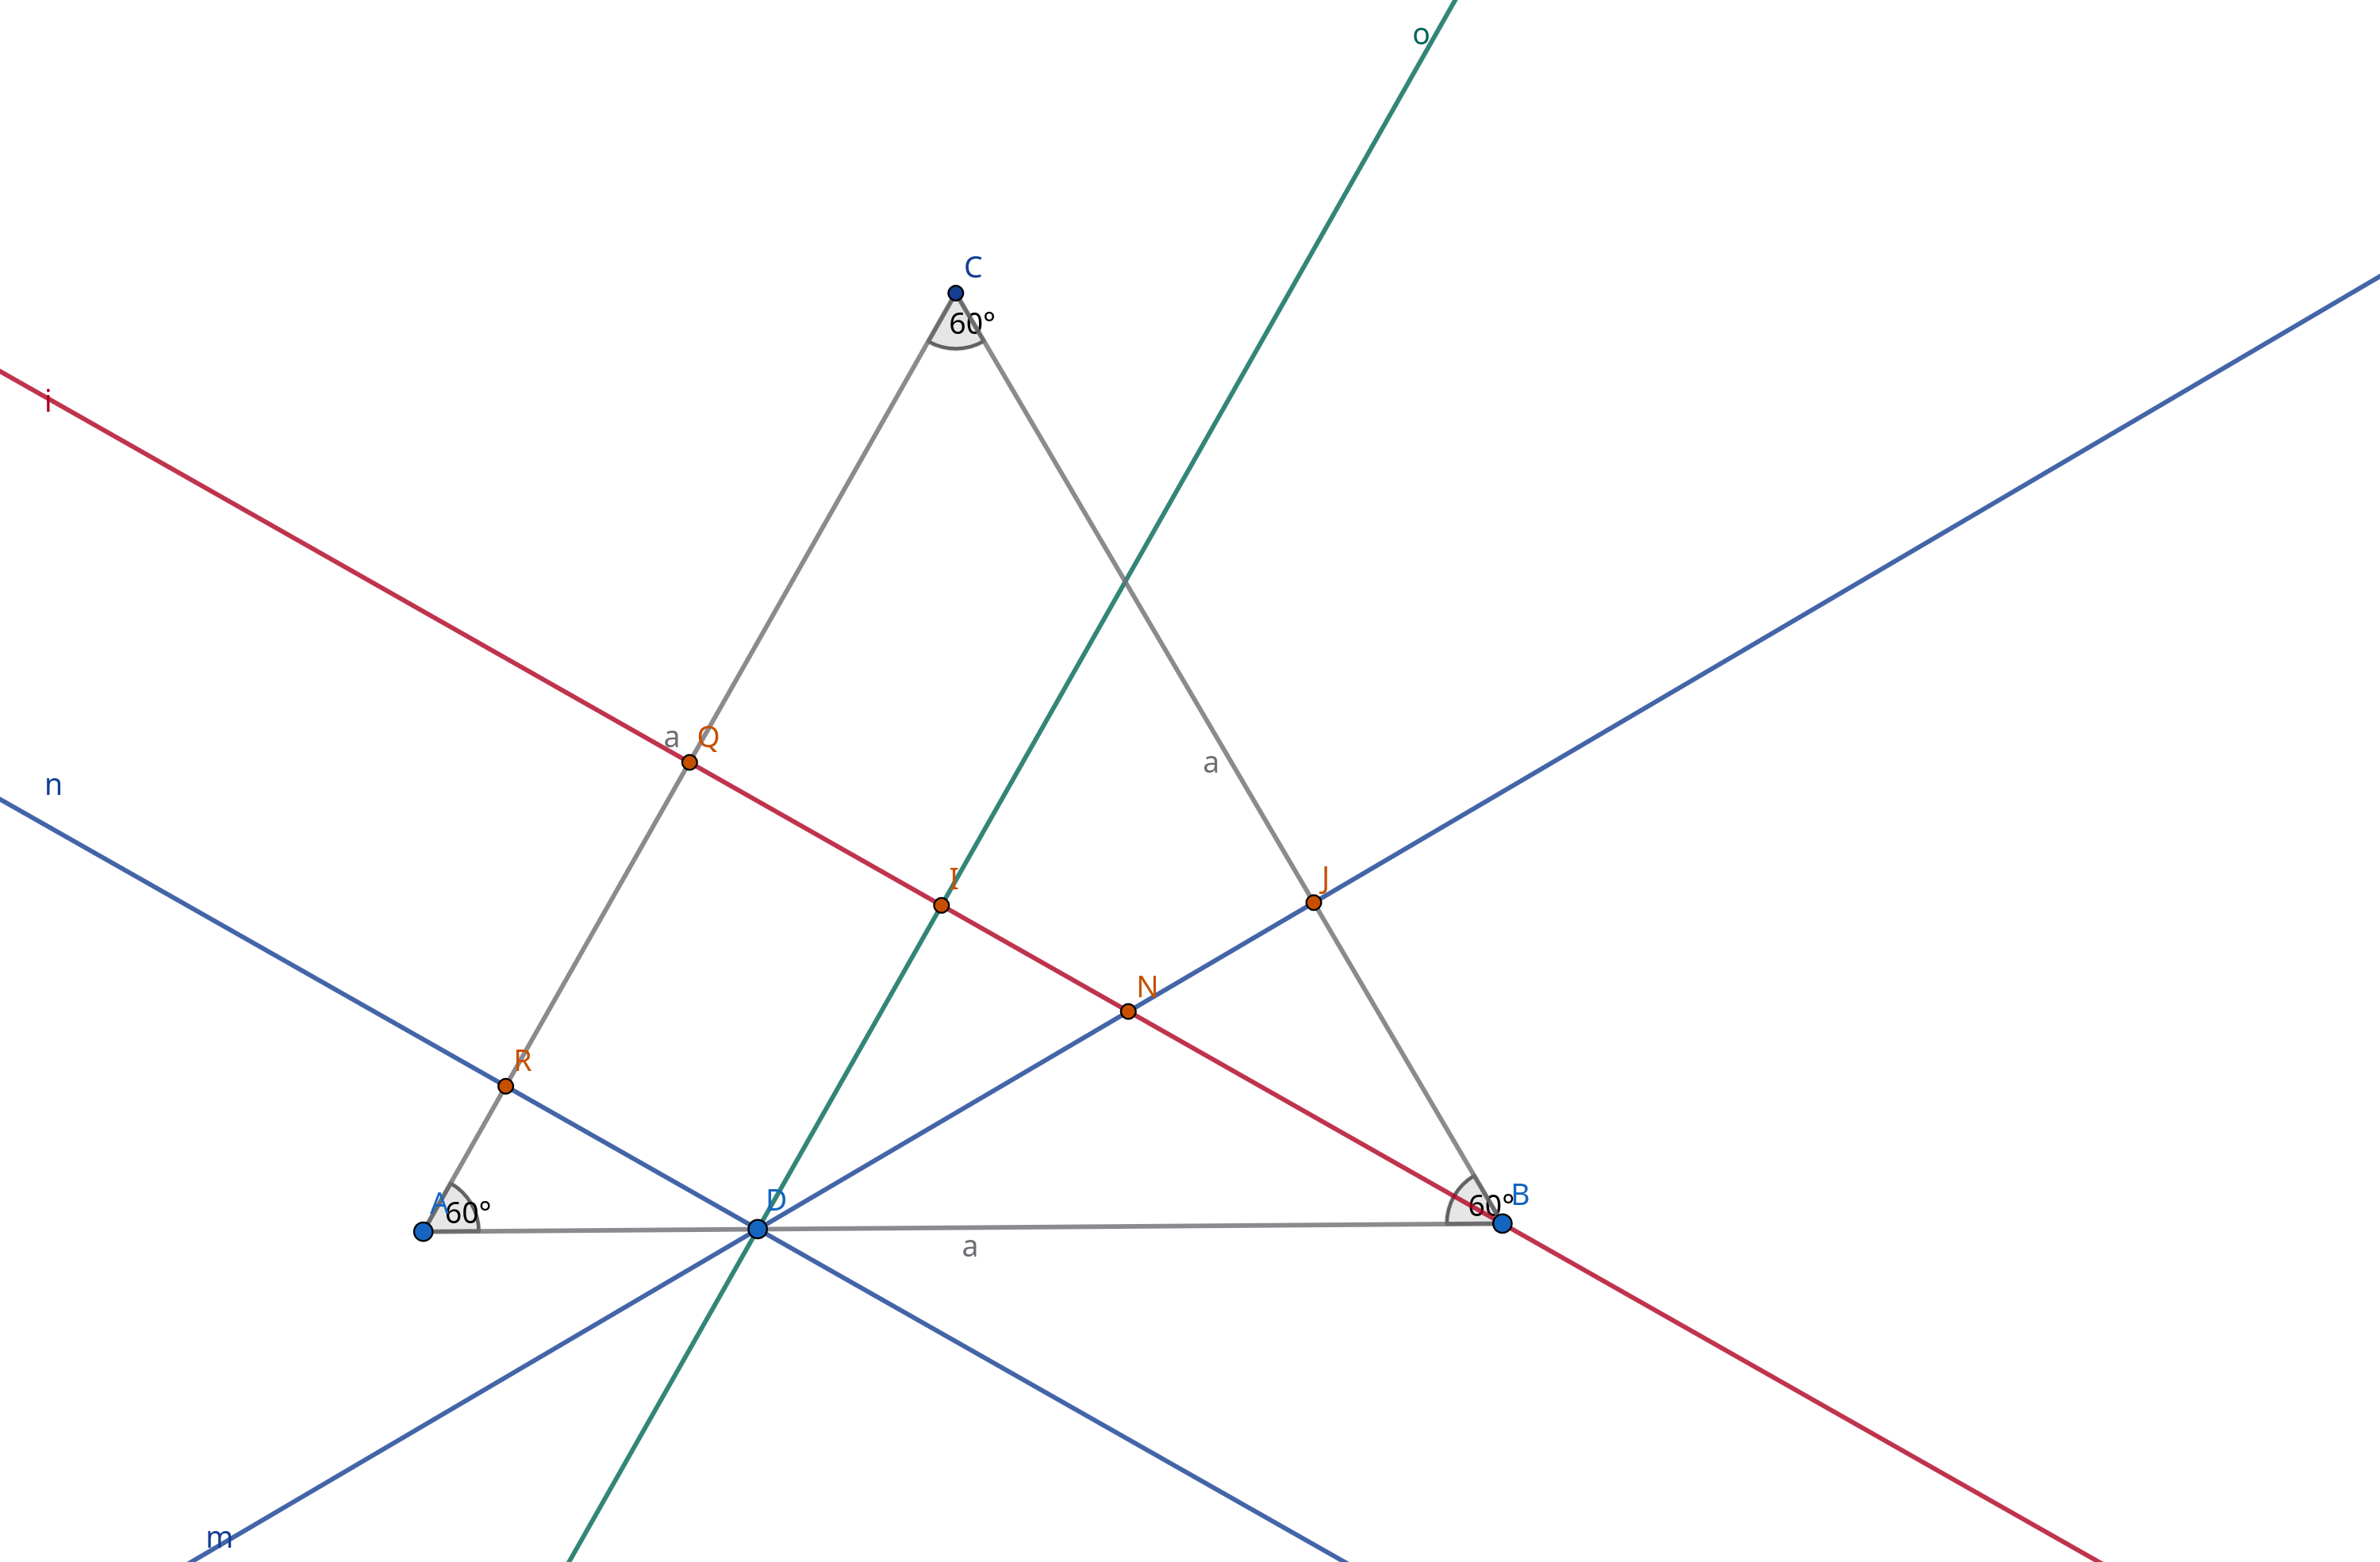
\includegraphics[width=0.8\textwidth]{Blatt03_Aufgabe_7_ii.png}
    \caption{Skizze}
    \label{fig:mein_bild}
\end{figure}

\noindent Sei $\triangle ABC$ ein gleichseitiges Dreieck.\\
Sei $i$ eine senkrechte Gerade zu $AC$ durch $B$.\\ 
Sei $m$ eine senkrechte Gerade zu $BC$ die $AB$ in einem Punkt  $D$ schneidet.\\
Sei $n$ eine senkrechte Gerade zu $AC$ die $AB$ im selben Punkt $D$ schneidet.\\
Sei $o$ eine parallele Gerade zu $AC$ durch $D$.\\ 
Sei $I$ Schnittpunkt von $o$ und $i$.\\ 
Sei $J$ Schnittpunkt von $m$ und $BC$.\\ 
Mit dem Stufenwinkelsatz gilt: $\angle DIB = 90^\circ$\\ 
Mit der Winkelsumme im gleichseitigen Dreieck: \\ 
$\angle ABC = \angle BCA = \angle CAB = 60\degree$\\ 
Nach Stufenwinkelsatz gilt: $\angle CAB = \angle IDB = 60^\circ$\\ 
Sei weiter $N$ Schnittpunkt von $m$ und $i$.\\ 
Da $\triangle ABC$ nicht entartet ist, muss $m \nparallel i$ sein, somit exisitiert N.\\
Nach Scheitewinkelsatz ist $\angle DNI = BNJ$. \\
Somit ist $\angle NBJ = \angle IDN$. Also sind $\triangle DBJ$ und $\triangle DBI$ kongruent.\\
$y = |DJ| = |BI|$.\\
Sei Q Schnittpunkt von AC mit i.
Sei R Schnittpunkt von AC mit n.
Durch Abstand von Parallelen, ist $|QI| = |RD| = x$\\
Woraus folgt $h = |QB| = |QI| + |IB| = x + y$.

\section*{Aufgabe 8}
\subsection*{(i)}
Hier muss ich gestehen, dass ich die Formulierungen nicht eindeutig interpretieren kann. Auf Wikipedia steht unter "Berechnung eines beliebigen Dreiecks" (\url{https://de.wikipedia.org/wiki/Dreieck}), das man WWW ohne Angabe einer Seite nicht lösen kann. Jedoch würde ich sagen, man ist in einer Seite Variabel und erhält durch jede Wahl ein anderes Dreieck. Man hat also unendlich viele nicht kongruente Dreiecke als Lösung. \\
Bei (a) gehe ich mal von einem Fehler aus, da ich mir das nicht anders vorstellen kann. Wenn ein Schüler ein Dreieck zeichnet und keinen Fehler bei der Angabe der Größen macht, dann exisitert dieses Dreieck und es kann nicht sein das man dieses Dreieck nicht konstruieren kann, da es ja schon konstruiert wurde.\\

\subsubsection*{(a)}
Eine Möglichkeit wäre, $\angle BCA = 90\degree$; $|AB| = 5cm$; $|BC| = 6cm$.\\
Da $\angle BCA = 90\degree$ hat, muss $AB$ die längste Seite sein, ist es aber nicht.

\subsubsection*{(b)}
$\angle BCA = 90\degree$; $\angle CAB = 60\degree$; $\angle ABC = 30\degree$. \\ 
Wenn man drei Winkel angibt, kann man eine Seitenlänge beliebig wählen und erhält dann die anderen zwei Seitenlängen. Man ist also Variabel in einer Seitelänge und erhält für jede unterschiedliche Wahl ein anderes Dreieck. Diese Dreiecke erfüllen keinen der Kongruenzsätze, da bei Kongruenten Dreiecken SSS gilt.

\subsubsection*{(c)}
$\angle \alpha = 40\degree$; $a = 3cm$; $b = 4cm$.
Wenn man zwei Seiten angibt und einen Winkel und dieser Winkel nicht der größeren der beiden Seiten gegenüberliegt, sondern der kleineren Seite gegenüber, gibt es meist zwei Dreiecke die man dann konstruieren kann. Es gibt jedoch einen Sonderfall wenn das Seitenverhältnis 1:2 und der Winkel $30\degree$ hat. Dann gibt es nur ein solches Dreieck.\\
\newpage
\subsection*{(ii)}
\begin{figure}[htbp]        
    \centering        
    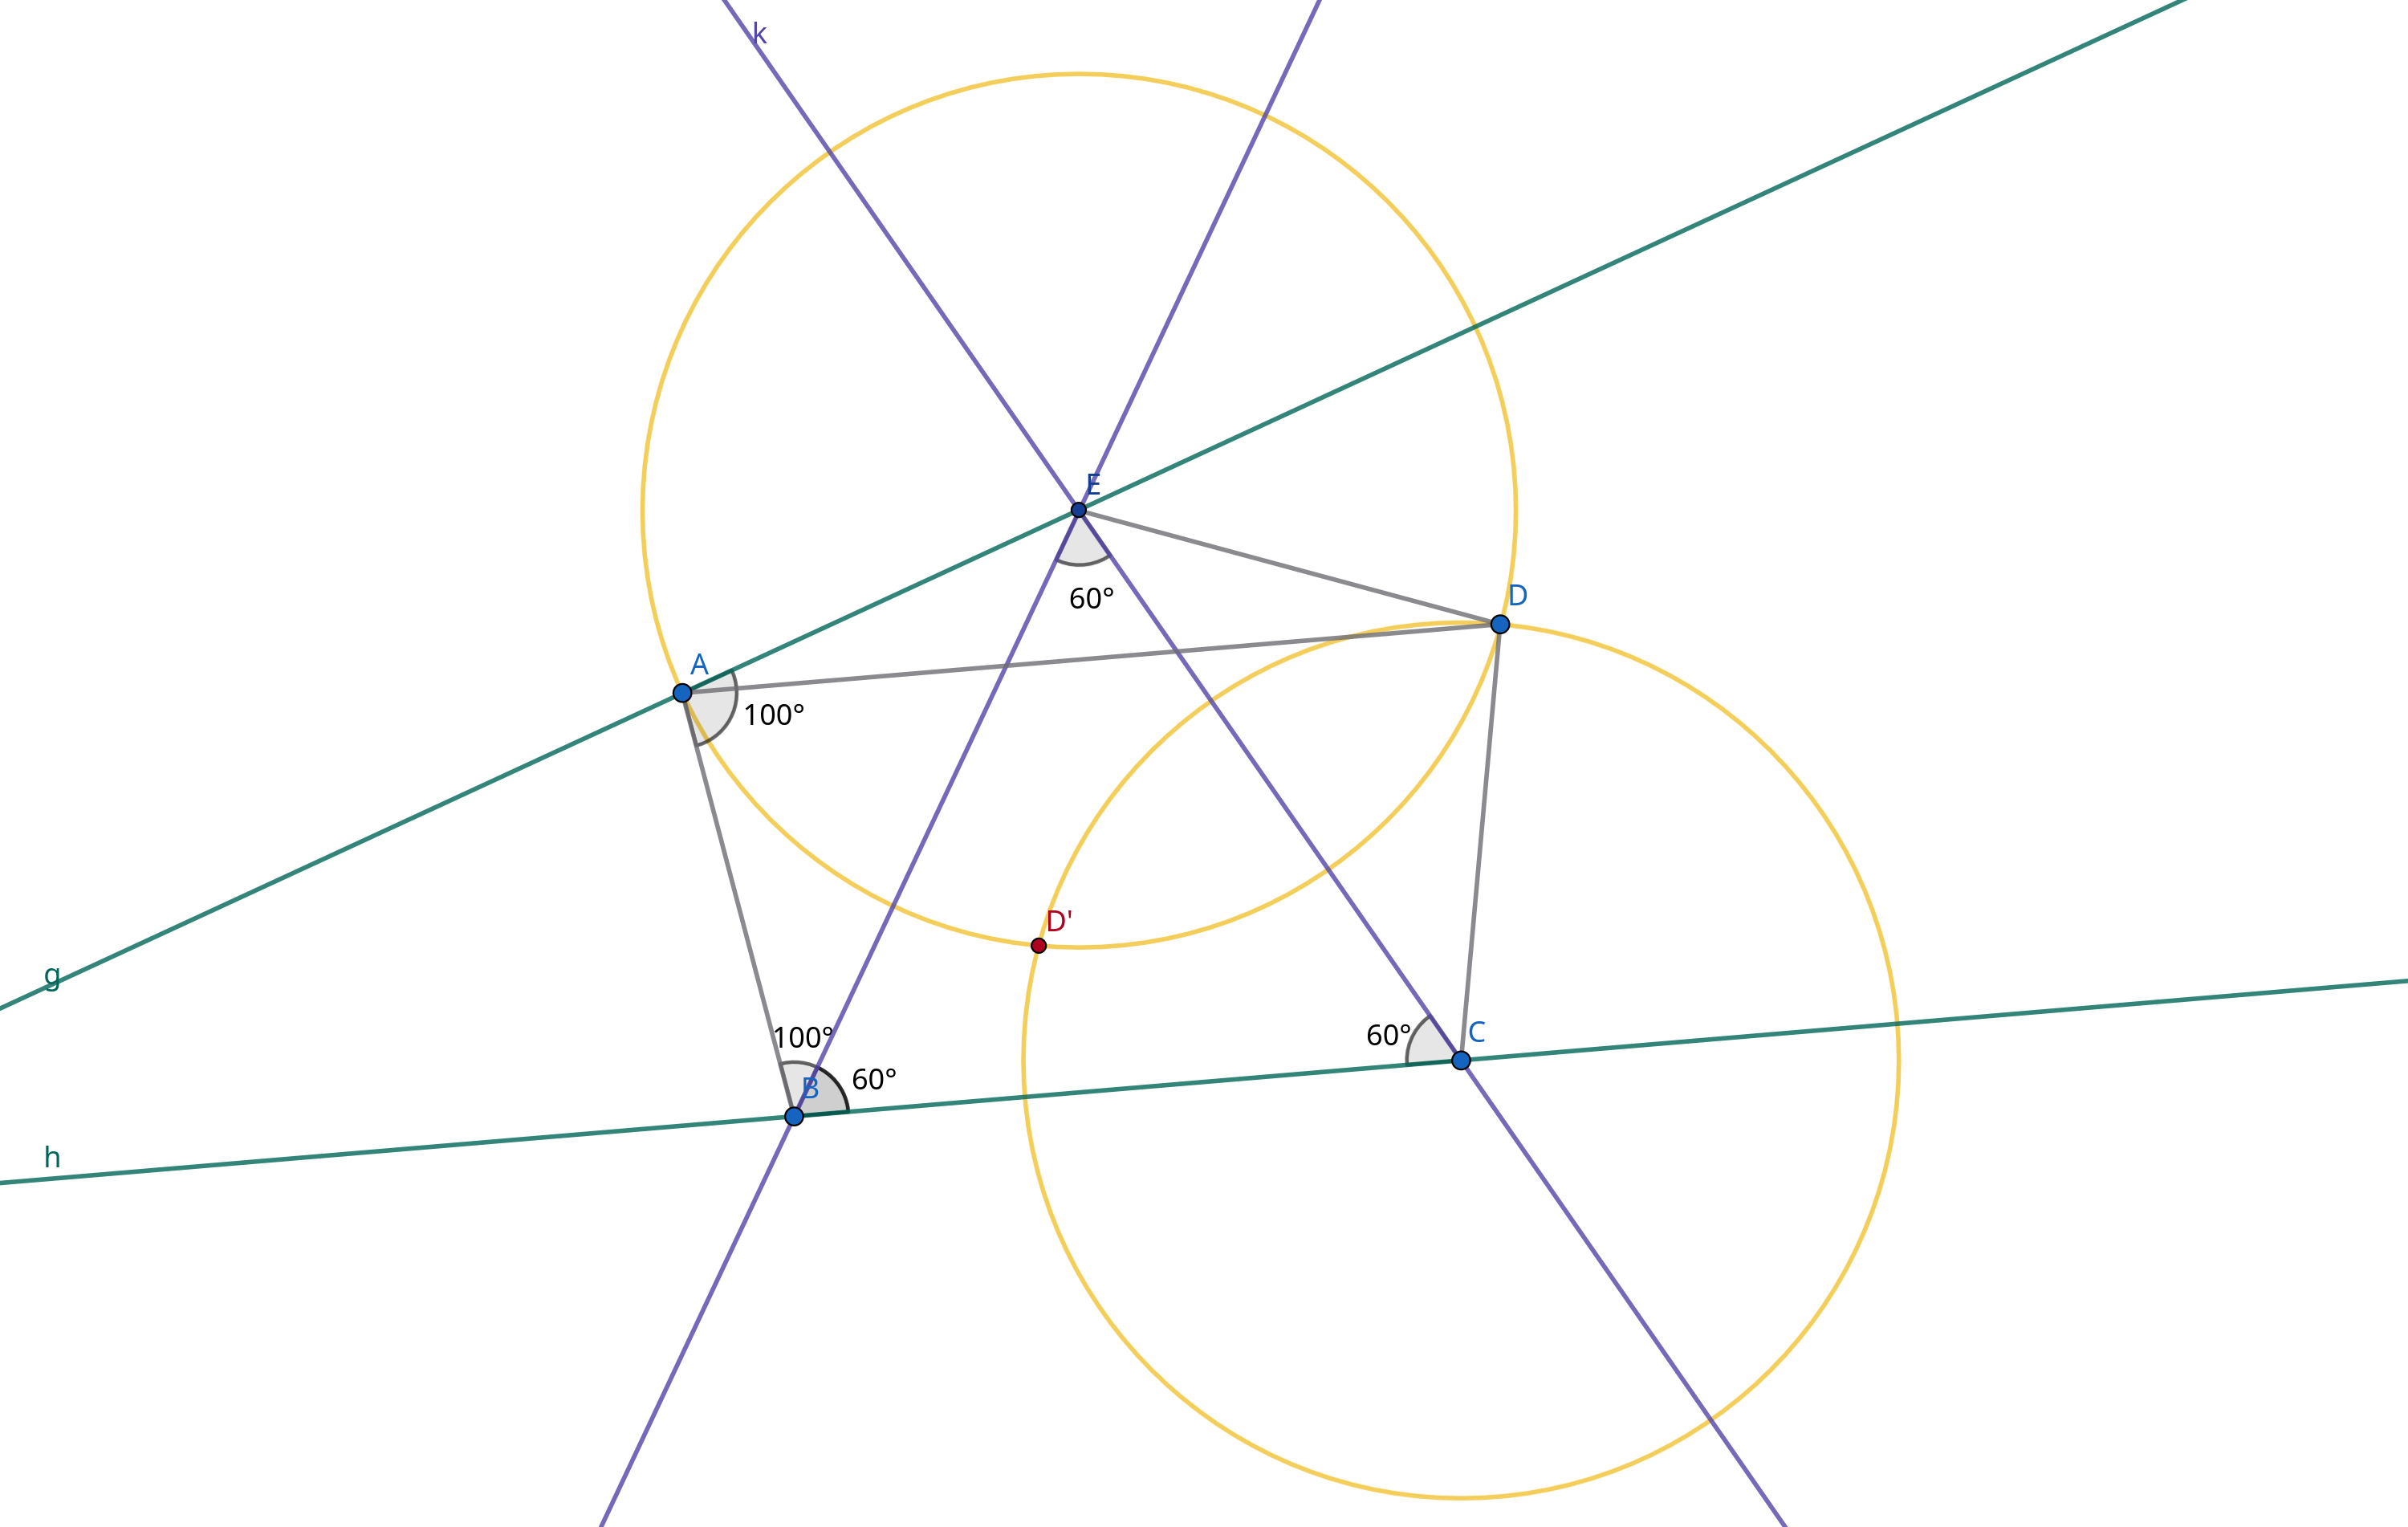
\includegraphics[width=0.8\textwidth]{Blatt03_Aufgabe_8_ii.png}
    \caption{Skizze}
    \label{fig:mein_bild}
\end{figure}

\noindent Dieses konvexe Fünfeck existiert und ist eindeutig.\\
 Zuerst zeichnet man die Punkte A und B ein mit |AB| = 6cm. Durch $\angle EAB = \angle ABC = 100\degree$ erhält man zwei Geraden g und h, auf diesen müssen E und C liegen.\\
Aus $|BC| = |CE| = |BE|$ weiß man, dass $\triangle BCE$ ein gleichseitiges Dreick ist und $\angle EBC = \angle BCE = \angle CEB = 60\degree$. Also kann man von der Geraden h eine weitere Gerade j einzeichnen, welche mit h einen $60\degree$ Winkel einschließt und durch B geht. E muss nun auch auf dieser Geraden liegen, ist also Schnittpunkt von j und g und somit eindeutig. \\
Von dieser Geraden j aus kann man nun wieder eine Gerade k einzeichnen die mit j einen $60\degree$ Winkel einschließt und durch E geht. C muss auf der Geraden k und auf der Geraden h liegen, ist also wieder Schnittpunkt und somit eindeutig.\\
Da nun E und A eindeutig sind, kann man einen Kreis mit Mittelpunkt E durch A einzeichnen. D muss wegen |DE| = |AE| auf diesem Kreis liegen. Da |DC| = 6cm, kann man einen Kreis mit Mittelpunkt C und Radius 6cm einzeichnen. Diese zwei Kreise haben zwei Schnittpunkte, D und D'. Da jedoch das Fünfeck nur für D und nicht für D' konvex ist, ist auch der Punkt D eindeutig. Alle Punkte sind eindeutig und somit ist das Fünfeck eindeutig.\\

\newpage
\section*{Aufgabe 9}
\subsection*{(i)}
\subsubsection*{(a)}
Hier scheinte die Methode der Höhenbestimmung eines Baumes mit dem Förster-Dreieck gemeint zu sein. Man nimmt sich ein gleichschenkliges Dreieck was zusätzlich einen rechten Winkel hat. Dann hält man das Dreieck so, dass man entlang der Hypotenuse den Wipfel des Baumes anschaut bzw man schaut entlang der Hypotenuse und bewegt sich solange auf den Baum zu oder weg vom Baum bis man den Wipfel sieht. Sei nun a der Abstand den man vom Baum hat. Man hat nun zwei ein gleichschenkliges Dreieck konstruiert und es ist:\\
h = f + a, wobei f und a bekannt sind.

\subsubsection*{(b)}
Hier macht man im Prinzip genau das Gleiche. Man nimmt sich wieder ein gleichschenkliges Dreieck mit rechtem Winkel. Man stellt sich an den Rand der Klippe und peilt über die Hypotenuse das Heck des Botes an. Man geht wieder soweit zurück vom Rand der Klippe bis man das Heck über die Hypotenuse angepeilt hat und misst wie viel man vom Rand der Klippe entfernt ist. Sei dies wieder der Abstand a. Man hat wieder ein gleichschenkliges Dreieck konstruiert und es ist: \\
H + g = a + w, wobei H, g und a bekannt sind.

\subsection*{(ii)}
\subsubsection*{(a)}
Da $\angle CAH_C = \angle CAB$ und $\angle AH_CC = \angle BCA$ sind die Dreiecke $\triangle ABC$ und $\triangle AH_CC$ änhlich. Es gilt $\frac{q}{h} = \frac{h}{p}$ was äquivalent ist zu $h^{2} = pq$.

\subsubsection*{(b)}
Da $\angle ABC = \angle H_CBC$ und $\angle BCA = \angle CH_CB$ sind die Dreiecke $\triangle ABC$ und $\triangle H_CBC$ ähnlich. Es gilt $\frac{c}{a} = \frac{a}{p}$ was äquivalent ist zu $a^{2} = pc$.

\subsubsection*{(c)}
Aus dem Höhensatz und dem Kathetensatz folgt:\\
$a^{2} + b^{2} = pc + qc = (p + q)c = c^{2}$.

\subsection*{(iii)}
Die Gewichtskraft ist $F_G = 120 kg \cdot 9,81 \frac{m}{s^{2}} = 1177,2 \frac{kg \cdot m}{s^{2}}$.\\
Mit dem Satz des Pythagoras aus (ii) lässt sich die Hypotenuse berechnen: \\
$c = \sqrt{l^{2} + h^{2}} = \sqrt{1,84m^{2} + 0,43m^{2}} \approx 1,89m$. \\
Die Hangabtriebskraft ist $F_{GH} = F_G \cdot \frac{h}{c} \approx 1177,2 \frac{kg \cdot m}{s^{2}} \cdot \frac{0,43m}{1,89m} \approx 267,98 \frac{kg \cdot m}{s^{2}}$. \\
Die Normalkraft ist $F_{GN} = F_G \cdot \frac{l}{c} \approx 1177,2 \frac{kg \cdot m}{s^{2}} \cdot \frac{1,84m}{1,89m} \approx 1146,36 \frac{kg \cdot m}{s^{2}}$.
\end{document}
